\documentclass[border=6pt]{standalone}
\usepackage{tikz}
\usetikzlibrary{arrows.meta}
\begin{document}
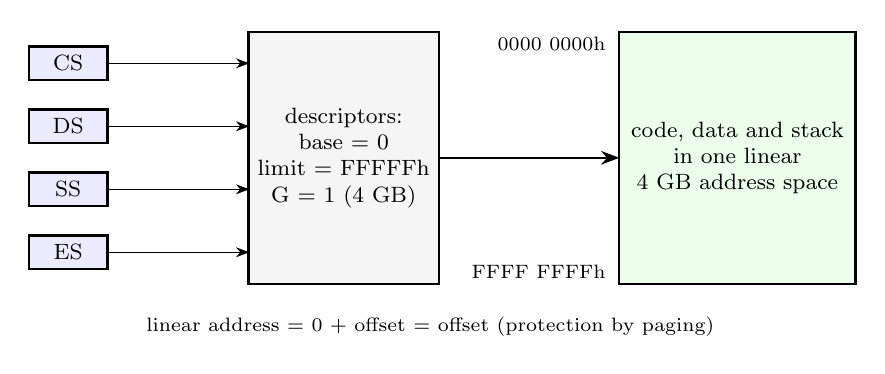
\begin{tikzpicture}[>=Stealth,font=\small]
\foreach \r/\y in {CS/1.6,DS/0.8,SS/0.0,ES/-0.8} {
  \node[draw,thick,fill=blue!8,minimum width=1.0cm,font=\footnotesize] (\r) at (0,\y) {\r};
  \draw[->] (\r.east) -- (2.3,\y);
}
\node[draw,thick,fill=gray!8,minimum height=3.2cm,minimum width=2.4cm,align=center,font=\footnotesize] (d) at (3.5,0.4) {descriptors:\\base = 0\\limit = FFFFFh\\G = 1 (4 GB)};
\draw[thick,fill=green!8] (7.0,2.0) rectangle (10.0,-1.2);
\node[font=\footnotesize,align=center] at (8.5,0.4) {code, data and stack\\in one linear\\4 GB address space};
\node[font=\scriptsize,anchor=east] at (6.95,1.85) {0000 0000h};
\node[font=\scriptsize,anchor=east] at (6.95,-1.05) {FFFF FFFFh};
\draw[->,thick] (d.east) -- (7.0,0.4);
\node[font=\scriptsize,anchor=north] at (4.6,-1.5) {linear address = 0 + offset = offset (protection by paging)};
\end{tikzpicture}
\end{document}
